\documentclass[12pt]{article}
\usepackage[labelfont=bf]{caption}
\usepackage{enumitem}
\usepackage[T1]{fontenc}
\usepackage[utf8]{inputenc}
\usepackage[a4paper,margin=0.75in]{geometry}
\usepackage{times}
\usepackage[parfill]{parskip}
\usepackage{lipsum}
\usepackage{afterpage}
\usepackage{fancyhdr}
\usepackage{array}
\usepackage{booktabs}
\usepackage{tabularx}
\usepackage{makecell}
\usepackage[numbers,sort&compress]{natbib}
\usepackage{graphicx}
\usepackage{pdflscape}
%\usepackage{anyfontsize}
\usepackage{microtype,newspaper,multicol,picinpar,newspaper-mod}
\usepackage{url}
\usepackage{float}

\pagestyle{fancy}
\fancyhf{}
\setlength{\headheight}{32.09pt}
\lhead{Page \thepage \hspace{1pt} of 25}
\rhead{Team \# 11682}

\graphicspath{ {./src/} }

\begin{document}
\afterpage{
\newgeometry{left=0.5in,right=0.5in,top=0.2in,bottom=0.5in}
\begin{centering}
    Team Control Number

    {\Huge 11682}

    Problem Chosen

    {\Huge \textbf{A}}

    {\Large \textbf{2021}}\\
    {\textbf{HiMCM/MidMCM}}\\
    {\textbf{Summary Sheet}}\\~\\

\end{centering}
\makebox[\textwidth]{\rule{\textwidth}{0.6pt}}
\begin{centering}
    (Your team's summary should be included as the first page of your electronic submission.)\\
    Type a summary of your results on this page. Do not include the name of your school, advisor, or team members on this page.

\end{centering}
Recently, solar power has become a popular alternative energy source. As more people begin the transition to renewable sources of energy, the need for more accessible information steadily rises. The typical solar energy systems includes four crucial parts : the panels, inverters, racking and solar battery storage units. However, installing battery banks for use when there is no sunlight remains a big problem for homeowners. Choosing the wrong type of battery leads to either insufficient wattage output, which makes generators or an external power grid necessary, or too much money spent on solar batteries. As such, those intending not to rely on the local electrical grid need to determine the number and type of battery they should install depending on their needs and budgets. Our mathematical model aims to address the following problem, establish the most effective way to set up battery arrays, in addition to analysing cement batteries. 

To start with, we identified a list of electrical appliances, along with their power ratings and the average number of hours used for each appliance. Each power rating is then multiplied by the number of hours used, before summing up to get the total energy used per day. 

Then, to find the "best" battery to use in a battery storage system, our team divided the model into two parts. The first part contains information about multiple batteries, with each battery having different electrical specifications. This section aims to establish aspects of the battery that needs to be taken into consideration. The second part finds the "best" battery to be used in a battery array through a rating system: multiple factors are evaluated, with each factor having different weights. These factors are then combined into a general rating, which allows the assessment of various batteries. 

As different types of batteries possess distinctive specifications, batteries having different chemical compositions and specifications can be compared using our method. Therefore, this model can be extended to any type of battery, hence it is easily adjustable to personal needs. For instance, different lengths of autonomy, energy consumption and state of health return different results when charting each battery’s rating on a bar chart. However, the model should only be consulted as reference material, and not a definitive tool to purchase a particular type of battery to install in a photovoltaic system. 

Finally, a recently developed technological advancement known as cement battery is addressed and evaluated after our model. We explored multiple advantages and disadvantages of the battery; in addition, we also designed a way to incorporate the battery in the house and other factors to consider before we can apply our mathematical model to the battery. By assessing the cement battery thoroughly, our team can evaluate its potential if it is used for solar energy storage, as cement batteries can be installed in walls, saving up space normally used by currently available batteries.
\clearpage
\restoregeometry
}

\tableofcontents
\newpage

\section{Introduction}
\subsection{Introduction}
Batteries are important components in a stand-alone photovoltaic system. It allows the storage of excess solar energy, provides energy for appliances during the night or non-sunny days, and also acts as a stabiliser by providing constant voltage to the loads. The most commonly used batteries nowadays are lead-acid batteries, though lithium-ion batteries are becoming an increasingly popular option. Batteries are one of the most complex elements in a PV system as many phenomena may occur, such as discharge and efficiency. Many parameters vary during a charge/discharge cycle: voltage, current, resistivity, temperature, et cetera. This leads to difficulties when predicting and simulating such a system. As a result, many homeowners struggled to choose their battery storage system and set up one in their house. Since there are many factors to consider, many stand-alone photovoltaic systems either invest too much money on batteries or too little, which leads to frequent power shortages. Therefore, our team aims to answer the following question: what is the "best" battery storage system for an off-grid home.

To answer this question, we have done in-depth research into the problem, developed a flexible and adaptable mathematical model, and provided a comprehensive and insightful analysis regarding the implementation of battery arrays in solar systems.

\subsection{Restatement of Problem}
\begin{enumerate}

\item Find the optimal arrangement in your 1600 square-feet home.

\begin{enumerate}
    \item Create a schedule for each electrical appliance's energy use in addition to a list of electrical devices.
    \item Develop mathematical models (or algorithms) describing your battery array choice on your stand-alone photovoltaic system.
    \item Discuss your selection on the "best" battery option based on the following chart and any additional information.
\end{enumerate}

\item Discuss any changes to the model from Subtask 1 that would be required to determine the optimal set-up for any homes which satisfy any personal needs.
\item Consider the possibilities of cement batteries.

\begin{enumerate}
    \item Discuss the benefits and drawbacks of the technology. Describe how you can implement it in your home.
    \item Identify additional data required to develop a model and compare the use of cement batteries.
\end{enumerate}

\item Write a news article discussing your team's model and potentials of cement batteries in the future.

\end{enumerate}


\section{Definitions and Assumptions}
\subsection{Glossary}
\begin{tabularx}{\textwidth}{lX}
    \specialrule{0.5pt}{0pt}{0pt}\toprule
    \bf Terms in the paper & \bf Definition\\
    \specialrule{0.75pt}{0pt}{0pt}\midrule
    Photovoltaic System & A system composed of one or more solar panels, combined with an inverter and other electrical devices that captures energy from the Sun to generate electricity\\
    \midrule
    Off-the-grid & Not using and being dependent on an external electrical grid\\ 
    \midrule
    Energy Storage System & A storage system that incorporates one or more batteries to capture electricity and store it for later uses\\
    \midrule
    Usable Capacity & The amount of electricity that can be drawn from batteries to power your home\\
    \midrule
    Round-Trip Efficiency & How much charge is retained when transmitting electricity through a circuit\\
    \midrule
    Lifetime (of battery) & The number of years or charge/discharge cycles a battery can undergo while still retaining its original capacity\\
    \midrule
    Instantaneous Power Rating & The maximum wattage the battery can deliver in a short period of time\\
    \midrule
    Continuous Power Rating & The maximum power the battery can deliver for multiple electric devices for a period of time\\
    \midrule
    State of Health & The difference in the capacity between a used battery and a fresh one\\
    \midrule
    Depth of Discharge & The capacity that is discharged from a fully charged battery, divided by battery nominal capacity\\
    \specialrule{0.25pt}{0pt}{0pt}\bottomrule
\end{tabularx}

\subsection{Variables}
\begin{tabularx}{\textwidth}{lX}
    \specialrule{0.5pt}{0pt}{0pt}\toprule
    \bf Variables & \bf Definition\\
    \specialrule{0.75pt}{0pt}{0pt}\midrule
    $L_a$ & Length of Autonomy\\
    \midrule
    $SoH$ & State of Health\\
    \midrule
    $DoD$ & Depth of Discharge\\
    \midrule
    $E_\text{daily}$ & Energy consumed daily\\
    \specialrule{0.25pt}{0pt}{0pt}\bottomrule
\end{tabularx}
\subsection{Assumptions \& Justifications}
\begin{enumerate}
    \item The house is 2-storey tall with a pitched-roof bungalow, and the batteries will be fully charged at the end of a sunny day
\end{enumerate}
By choosing a 2-storey tall pitched-roof bungalow, we can maximise the energy output of each solar panel, thus ensuring that each battery has maximum charge at the end of the day (i.e. no more energy from the sun can be harvested). 
\begin{enumerate}[resume]
    \item Calculations will be done in winter
\end{enumerate}
Winter is generally the worst-case scenario since the duration of sunlight will be less compared to the rest of the year, and electricity consumption will be highest. Usage of energy-intensive appliances in winter (e.g. boilers, electric heaters) is generally higher than the usage of those in summer (i.e. air conditioning).
\begin{enumerate}[resume]
    \item There will be days without or with little sunlight (i.e. due to blizzards, overcast, etc.)
\end{enumerate}
This is to consider special occasions when there is no sunlight, in which the number of days of autonomy has to be taken into account, for little solar energy is harvested. By estimating the average length of autonomy, we can ensure the system will be capable of supporting the house even when solar panels cannot harvest energy.
\begin{enumerate}[resume]
    \item Batteries start charging when the house is vacant, and stop when everyone is at home.
\end{enumerate}
During the morning, when the weather is sunny, the batteries will start charging, thus reaching maximum capacity at the end of the day. Otherwise, there will be no net gain; hence, the batteries will expend their energy stored inside.

\section{Energy demands}
\subsection{Additional factors}
After analysing requirement (1.a) thoroughly, we have constructed our answer to the energy demands in the 1600-square-foot home. There are many factors to consider; hence, before making a list of electrical appliances, we need to answer several questions in regards to the electrical needs of the family members residing in the house:
\begin{enumerate}
    \item The number of family members living in the house
\end{enumerate}
As the average size of an American household is four people, we have decided that the family will consist of two parents, a son and a daughter. This will most likely be the household that consumes the most electricity, as each person will require different energy demands in the house.
\begin{enumerate}[resume]
    \item The charge/discharge cycle of the batteries
\end{enumerate}
Our team assumed that the batteries start charging when there is no one in the house; only appliances that constantly operate which are fridges and security cameras are powered. The batteries will stop charging when everyone is at home using electrical appliances. In addition, we assume that everyone will either start going to school or commuting to work at 8:30 a.m., and everyone is presented at home at 5:30 p.m. when the sun begins to set during the winter months. Therefore, the average number of hours when the batteries discharge is 15 hours.
\begin{enumerate}[resume]
    \item Electricity consumption and power ratings
\end{enumerate}
Since different electric appliances require different needs, by researching the average wattage and hours used per device, we can calculate the mean electricity consumption per day. By multiplying the appliance's wattage with the number of hours used, we get the average energy used by the appliance per day. These values will be summed up, which will return the total amount of energy required to power these devices for the day.
\subsection{Electrical appliances}
We have developed a list of electrical devices, their accumulated hours, and the average usage per device to calculate the energy needs per day for our model based on the following website\cite{daft:power}:
\begin{table}[H]
  \caption{Electrical appliances and their energy demands}
    \begin{tabular}{|c|c|c|c|c|c|}
    \toprule
    Appliances & \multicolumn{1}{p{4.955em}|}{Average Wattage} & \multicolumn{1}{p{4.91em}|}{Number of devices} & \multicolumn{1}{p{4.365em}|}{Hours per device} & \multicolumn{1}{p{8.5em}|}{Total accumulated hours per day} & \multicolumn{1}{p{4.365em}|}{Average usage} \\
    \midrule
    TV (49 - 55inch) & 100   & 1     & 3     & 3     & 300 \\
    \midrule
    fridge & 100   & 1     & 24    & 24    & 2400 \\
    \midrule
    oven  & 2150  & 1     & 1     & 1     & 2150 \\
    \midrule
    microwave & 600   & 1     & 0.3   & 0.3   & 180 \\
    \midrule
    stove & 2000  & 1     & 2     & 2     & 4000 \\
    \midrule
    stand mixer & 300   & 1     & 0.25  & 0.25  & 75 \\
    \midrule
    coffee maker & 800   & 1     & 0.3   & 0.3   & 240 \\
    \midrule
    toaster oven & 800   & 1     & 0.3   & 0.3   & 240 \\
    \midrule
    lights & 7     & 40    & 12    & 480   & 3360 \\
    \midrule
    dishwasher & 1200  & 1     & 2     & 2     & 2400 \\
    \midrule
    boiler & 4000  & 1     & 2     & 2     & 8000 \\
    \midrule
    vacuum cleaner & 450   & 1     & 0.25  & 0.25  & 112.5 \\
    \midrule
    washing machine & 500   & 1     & 1     & 1     & 500 \\
    \midrule
    phones & 4     & 4     & 1.5   & 6     & 24 \\
    \midrule
    computers & 30    & 2     & 2     & 4     & 120 \\
    \midrule
    security cameras & 4     & 5     & 24    & 120   & 480 \\
    \midrule
    iron  & 1000  & 1     & 0.1   & 0.1   & 100 \\
    \midrule
    hair dryer & 1800  & 1     & 0.3   & 0.3   & 540 \\
    \midrule
    lawn mower & 1000  & 1     & 0.2   & 0.2   & 200 \\
    \midrule
    pressure pump & 250   & 1     & 3.5   & 3.5   & 875 \\
    \midrule
    kitchen hood & 105   & 1     & 2     & 2     & 210 \\
    \midrule
    game console & 120   & 1     & 3     & 3     & 360 \\
    \midrule
    electric razor & 15    & 1     & 0.2   & 0.2   & 3 \\
    \midrule
    blender & 300   & 1     & 0.25  & 0.25  & 75 \\
    \midrule
    speakers & 100   & 2     & 1.5   & 3     & 300 \\
    \midrule
    dehumidifier & 240   & 1     & 12    & 12    & 2880 \\
    \midrule
     &       &       &       &       & 30124.5 \\
    \bottomrule
    \end{tabular}%
  \label{tab:tabl1}%
\end{table}%
\newpage
Despite this, the table above has not included multiple essential parameters presented in our model, including the power ratings of these appliances, though this will be addressed later in our mathematical model.

\section{Mathematical Model}
\subsection{Factors taken into consideration}
As said above, there are factors to consider when determining which battery storage system is the "best". Here we have included several important factors that our model use:
\begin{enumerate}
    \item Power rating
\end{enumerate}
In an AC circuit, the power rating determines the ability to discharge and supply enough power to electrical appliances. Therefore, by having a high power-rating, a battery can supply more electricity to more devices, making it an important factor when evaluating a battery system.
\begin{enumerate}[resume]
    \item Capacity of the battery storage system
\end{enumerate}
If the array's capacity is too low, the system will either struggle to power the entire home or have the depth-of-discharge higher than the recommended level. In that case, without another backup power grid, the system will shut down, leaving electric appliances in the house unusable, and the lifetime of the batteries will decrease.
\begin{enumerate}[resume]
    \item Length of autonomy
\end{enumerate}
In the worst-case scenario, there will be days without sufficient energy to charge the batteries up to full capacity. The system must not shut down during usage. Since weather patterns vary throughout the country, each customer will have specific demand of length of autonomy.
\begin{enumerate}[resume]
    \item Efficiency of the battery storage system
\end{enumerate}
It is unavoidable that some electricity transmitted through the circuit is wasted. Therefore, to retain as much charge as possible, the system's efficiency should be as high as can be achieved.
\begin{enumerate}[resume]
    \item Lifetime of a battery
\end{enumerate}
The lifetime of a battery describes both the number of years it can effectively charge and the number of cycles it can run when using at a certain depth of discharge. Since the lifetime of the battery is tied to the cost (the higher the lifetime, the average cost will be lower), it is considered to be an important factor in our model.
\begin{enumerate}[resume]
    \item Warranty of a battery
\end{enumerate}
The warranty of a battery describes the number of years a battery can last before losing too much capacity to charge and deliver electricity effectively. As this factor is tied to the lifetime of a battery, we have decided to include it in our mathematical model.
\subsection{Additional terms \& variables}
%\begin{tabularx}{\textwidth}{lX}
%    \specialrule{0.5pt}{0pt}{0pt}\toprule
%    \bf Terms in the paper & \bf Definition\\
%    \specialrule{0.75pt}{0pt}{0pt}\midrule
%    Statistics capacity & \\
%    \specialrule{0.25pt}{0pt}{0pt}\bottomrule
%\end{tabularx}

\begin{tabularx}{\textwidth}{lX}
    \specialrule{0.5pt}{0pt}{0pt}\toprule
    \bf Variables & \bf Definition\\
    \specialrule{0.75pt}{0pt}{0pt}\midrule
    $P_c$ & Continuous power rating\\
    \midrule
    $P_i$ & Instantaneous power rating\\
    \midrule
    $R_p$ & Average power rating\\
    \midrule
    $R_\text{cost}$ & Cost rating\\
    \midrule
    $R_\text{cap}$ & Capacity rating\\
    \midrule
    $R_g$ & General rating\\
    \midrule
    $N_c$ & Number of cycles\\
    \midrule
    $N_b$ & Number of batteries\\
    \midrule
    $C_a$ & Actual capacity\\
    \midrule
    $E_\text{daily}$ & Energy consumed per day\\
    \specialrule{0.25pt}{0pt}{0pt}\bottomrule
\end{tabularx}
\subsection{Additional assumptions \& justifications}
\begin{enumerate}
    \item The weight and dimension of the battery are not taken into account in the model
\end{enumerate}
As the model only considers  electrical specifications of the batteries, physical aspects (e.g. weight, dimension) will not be represented in the model. This is because each battery storage system's location is dependent on the house layout, and different house plans make it difficult to model the weight and dimension consistently.
\begin{comment}
\begin{enumerate}[resume]
    \item The battery array might be heterogeneous (i.e. having multiple types of batteries in the same system)
\end{enumerate}
In order to optimise both the cost and efficiency of the system, our team will test several layouts that make use of multiple types of batteries (i.e. lithium-ion batteries, lead-acid batteries, LFP batteries). The main reason for this is to evaluate the model more fairly, which helps us develop a stronger solution.
\end{comment}
\begin{enumerate}[resume]
    \item A day consists of a cycle
\end{enumerate}
Since electricity is consumed continuously in the evening and batteries are charged continuously in daytime, it is reasonable to assume that a day consists a charge/discharge cycle.
\subsection{Model Construction}
First, we need to analyse the specifications of different batteries. There are many brands and types of batteries commercially available. Therefore, before installing the batteries in our photovoltaic system, we need to consider our choices:
\begin{enumerate}
    \item Lead-acid batteries
\end{enumerate}
Lead-acid battery is the most popular and reliable chemistry used in a PV storage system, as it has been around since the 19th century. The stored chemical potential energy in the battery can be converted to electricity by the following reaction:

$$\mathrm{Pb}+\mathrm{PbO}_{2}+2 \mathrm{H}_{2} \mathrm{SO}_{4} \rightarrow 2 \mathrm{PbSO}_{4}+2 \mathrm{H}_{2} \mathrm{O}$$
$$
E^{0}=2.041 V
$$
, in which the voltage produced from the reaction is $2V$.\cite{wiki:lead_acid_battery}

\begin{enumerate}[resume]
    \item Lithium-ion batteries 
\end{enumerate}
Despite lithium-ion batteries being more expensive than their lead-acid counterparts, they are more efficient and allow more depth of discharge, thus being more cost-effective in the long run. Via separating the lithium ions from the electrons via an electrolyte, the electron can be directed through a circuit to discharge the chemical potential energy inside.\cite{wiki:li_ion_battery} \\

\begin{enumerate}[resume]
    \item Lithium iron phosphate (LFP) batteries
\end{enumerate}
LFP battery is a lithium-ion battery that uses lithium iron phosphate instead of lithium cobalt oxide as cathode material. While the energy density and nominal voltage of this type of battery are lower than that of a traditional lithium-ion battery, it is generally safer, cheaper, has a higher discharge rate and has a longer life cycle.\cite{wiki:lfp_battery}\\ 
With all of that in mind, we decided to choose 15 batteries, with 4 being lead-acid batteries, 11 being lithium-ion batteries, with 7 of which are lithium iron phosphate batteries. This is because we need to test a variety of batteries to find the most optimal choice between different batteries (see \textbf{Appendix} A for additional information).

However, it will be very difficult for people who have not worked with either batteries or electrical devices before to assess the following table to find the "best" battery. Our team determines that there should be a rating system that is easy to understand, convenient for users but also accurate during evaluation, making the process of choosing a suitable battery for solar energy storage easier. Here are several factors\cite{solar:guide} and formulas our team has taken into consideration and a model that assesses multiple battery storage systems:

\begin{enumerate}
    \item Power rating
\end{enumerate}
The following formula,
\begin{equation}
    R_p = \frac{P_c \times 59 + P_i}{60} \times \text{average usage per hour}
    \label{eq:-2}
\end{equation}
returns the average power rating concerning the continuous power rating, the instantaneous power rating and the average power consumed per hour. Within an hour, the device only reaches peak power usage for about one minute, with the rest consuming energy at a constant rate. Therefore, we can calculate the mean power by using the formula (59 * continuous power rating + instantaneous power rating), after which is then divided by the correct coefficient (60 minutes in an hour, 59 minutes of constant power usage and one minute of peak power consumption).

\begin{enumerate}[resume]
    \item Cost rating
\end{enumerate}
The cost rating is calculated through the following formula:
\begin{equation}
    C_r = \frac{\text{Cost}}{\text{Lifetime}} = \frac{\text{Cost}}{(N_c / 365)}
    \label{eq:-1}
\end{equation}
Because each battery has a different lifetime and cost, it can be hard to evaluate directly based on the original price. We believe that calculating the average cost per year spent on the system is a reasonable choice. As a day consists of a cycle on average, therefore the duration in which the battery system is used is approximately the number of cycles divided by 365 days in a year. From that, we can derive a formula to calculate the cost rating.

\begin{enumerate}[resume]
    \item Capacity rating
\end{enumerate}
The capacity rating is calculated as follow:
\begin{equation}
    R_\text{cap} = \frac{N_b \times C_a}{E_\text{daily} \times L_a} 
    \label{eq:0}
\end{equation}
As we mainly use the batteries when there is no sunlight, which invokes the length of autonomy (LoA), our battery system needs to store enough electricity to use during the duration of the LoA ($E_daily \times L_a$). We can calculate the amount of electricity stored in the system by multiplying the number of batteries by the battery's capacity. Therefore, to find the ratio between capacity, we use the formula above.
\begin{equation}
    \text{minimum } SoH = \frac{L_a \times E_\text{daily}}{N_b \times C_a \times DoD \times RTE}\label{eq:1}
\end{equation}
For the batteries to be utilised to their maximum potential, they need to supply enough electricity during a discharge cycle. Thus, the minimum state of health (in percent) can be calculated via the equation\eqref{eq:1} by dividing the total energy used for the entire duration of the length of autonomy by the amount of electricity the system can supply.
\begin{equation}
    SoH \text{ decreasing rate} = \frac{1 - \text{warranty } SoH}{365 \times \text{warranty length}}\label{eq:2}
\end{equation}
As batteries operate on an electrochemical basis, they will inevitably degrade over time. This value is represented by the state of health, which additionally is the capacity percentage of a used battery compared to an unused one. Many battery manufacturers include details on the warranty period of the battery in addition to the estimated state of health when the warranty expires. When the state of health falls under a certain threshold, its quality will decline as it cannot charge and supply enough electricity for home usage. From all of these values, we can calculate the average decreasing rate of the state of health via the equation \eqref{eq:2}, in which the warranty $SoH$ is the state of health of an unused battery and the warranty time is the number of years of warranty.
\begin{equation}
    \text{Expected }N_c = \frac{1 - SoH}{SoH \text{ decreasing rate}}\label{eq:3}
\end{equation}

After calculating the rate of degradation of the state of health, we can find the number of estimated cycles we can use through equation \eqref{eq:3}. This number of cycles is an important factor that affects the estimated lifespan of the battery system.

\begin{equation}
    \text{Lifetime} = \frac{\min{(\text{warranty cycle}, \text{expected }}N_c)}{365}\label{eq:4}
\end{equation}

Finally, equation \eqref{eq:4} calculates the lifespan of the battery system; the warranty cycle is the number of usable cycles based on the manufacturer's warranty, and the number of expected cycles is the number of times we estimated the battery to work in peak condition. But why do we have to take the minimum between the two? Besides the simple factors we have just calculated, the lifetime of a battery depends on other complex external factors; if we consider every single factor, the model will become too complicated. Therefore, our team will not address these problems since these variables are included in the specification sheet that comes with the battery.

After constructing a rating system for batteries, we found that it is necessary to have a general rating for everyone to refer to easily. Our team still utilises each criterion's rating to evaluate, although a general rating will allow customers to have a better insight into each battery to choose from. We calculate the general rating via each rating in different proportions. Nevertheless, before combining each rating, they need to have roughly the same value, as it is not feasible to merge a cost rating of \$350 per year with a power rating of 1.05. In light of this, our team decided to include additional variables. Since the mean power rating of each battery type lies within the range of 5 and 8, adding $\frac{1}{6}$ in front will help reduce the value to 1, making calculations easier. In addition, the cost rating is better the smaller it gets, so when contributing to the general rating, we will calculate its complement. We also divide the cost rating by 1000, as the average cost spent on solar batteries per year falls from \$900 to \$1000. Finally, all the ratings are combined with the proportions equivalent to this pie chart:

\begin{figure}[ht]
    \centering
    \begin{tikzpicture}
        \pie[text=legend,radius=2]{30/Power rating,
        40/Capacity rating,
        25/Cost rating,
        5/Warranty} 
    \end{tikzpicture}
    \caption{Proportion of each rating in the general rating}
\end{figure}

We can finally derive a general rating formula as follow:
\begin{equation}
    R_g = \frac{0.5R_p + 4R_\text{cap} + 2.5 \times (100\% - (R_\text{cost} / 1000)) + 0.5 \times \text{warranty rating}}{10}
\end{equation}

\section{Model evaluation}
\subsection{Advantages of model}
\begin{enumerate}
    \item Ease of use
\end{enumerate}
Our team designed a simple model catering to the general public, as other complex models will require a prior understanding of the inner workings of electrical circuits, which might prevent many people from learning this model.

\begin{enumerate}[resume]
    \item Flexibility
\end{enumerate}
Since our model depends on multiple factors, changing one or multiple variables can alter the model, giving different results. This can be incredibly useful when the conditions of the problem change as we have tested our model using different values. Therefore, the result will not be fixed, allowing users to have accurate and objective views on which battery type to choose.

\begin{enumerate}[resume]
    \item Applicable to other types of batteries
\end{enumerate}
Each battery will produce different parameters; however, the conversion of each parameter into a more general one (i.e., same capacity rating, cost rating) will make comparisons more feasible than making comparisons of two entirely different batteries.
\subsection{Drawbacks of model}
\begin{enumerate}
    \item Large margin of error
\end{enumerate}
A problem in the model is that the margin of error may be potentially larger than expected, or the calculating process may not be as accurate. Since the model ignores several small factors, a margin of error is inevitable.
\begin{enumerate}[resume]
    \item The model is relativistic
\end{enumerate}
Our model is for reference only, allowing users to assess different batteries using a rating scale but does not allow unabridged assessments among different types of batteries. Batteries with higher ratings might be better, but they might not necessarily suit one's budget or demands. However, we have developed recommended criteria for choosing the most suitable battery for one's home so that readers can decide.
\begin{enumerate}[resume]
    \item Several factors left out
\end{enumerate}
During our calculation process, several complex or unimportant factors have been left out. However, in certain cases, these factors might play more important roles. It would be difficult to assess their importance; hence we decided to leave them out. To make the most reasonable choice, one can still refer to our model and consider variables not presented in our model.

\section{Changes in model}
After constructing the following model, we decided to make some additional changes in the model as follow:
\begin{itemize}
    \item Initial parameters: area = 1600 sq. ft, $E_\text{daily} = 30kWh, L_a = 1$
\end{itemize}
\begin{figure}[H]
\centering
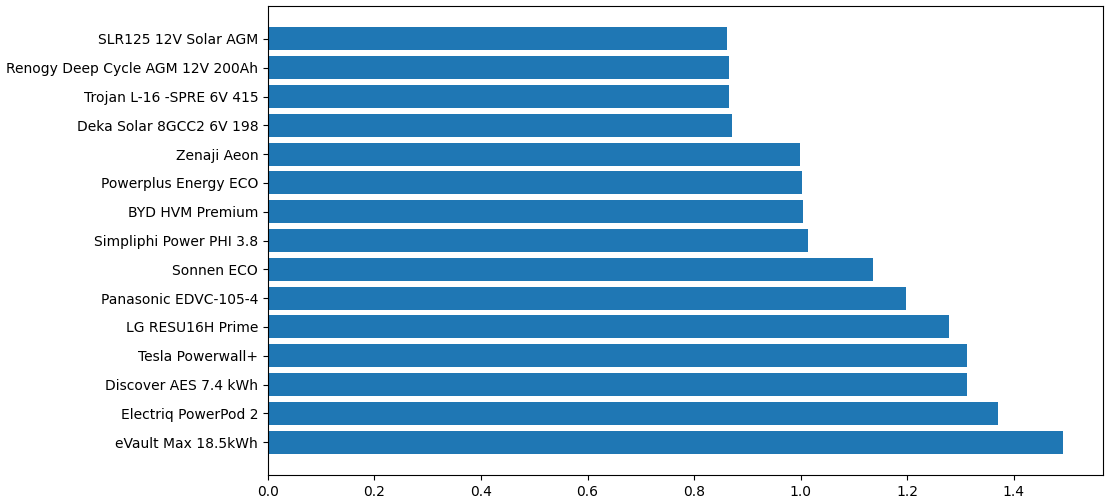
\includegraphics[scale=0.4]{src/1.png}
\end{figure}
By consulting the bar chart, one can see that there are several qualified batteries (i.e., Sonnen ECO). In addition, we also recognise batteries that have very high ratings but cannot be fully utilised (i.e., eVault Max 18.5kWh). However, it is not always the case when choosing a battery for our 1600 square-foot house. Therefore, we need to recalculate individual ratings when each factor changes. Here are several calculations on the general rating of several batteries when:
\begin{itemize}
    \item Reducing $E_\text{daily}$ to $25kWh$:
\end{itemize}
\begin{figure}[H]
\centering
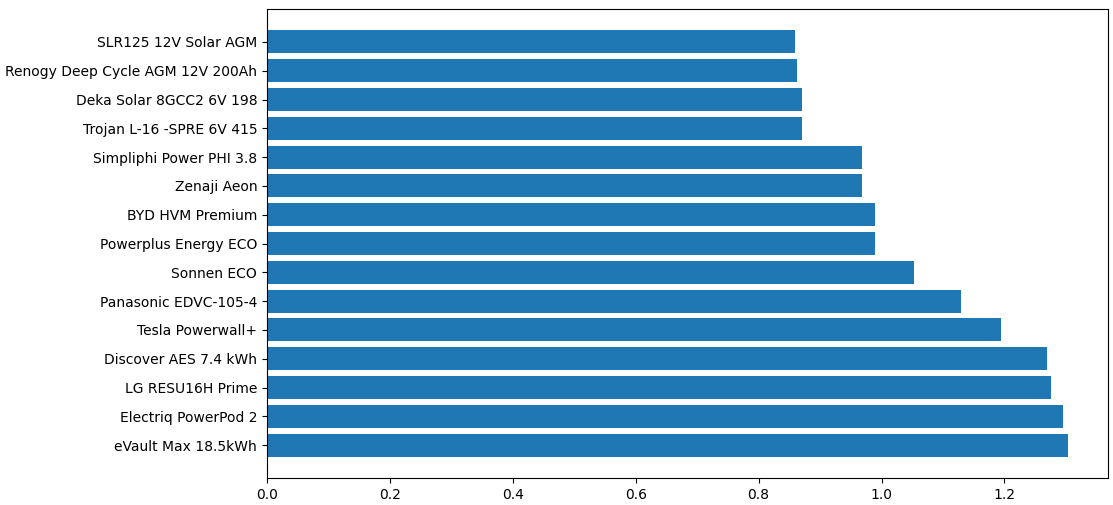
\includegraphics[scale=0.4]{src/2.png}
\end{figure}
$25kWh$ is the daily energy consumption in temperate climate areas when the weather is pleasant, and there is no demand for more electricity consumption. Therefore, the problem of choosing which battery to use will also change.
\begin{itemize}
    \item Increasing $E_\text{daily}$ to $45kWh$:
\end{itemize}
\begin{figure}[h]
\centering
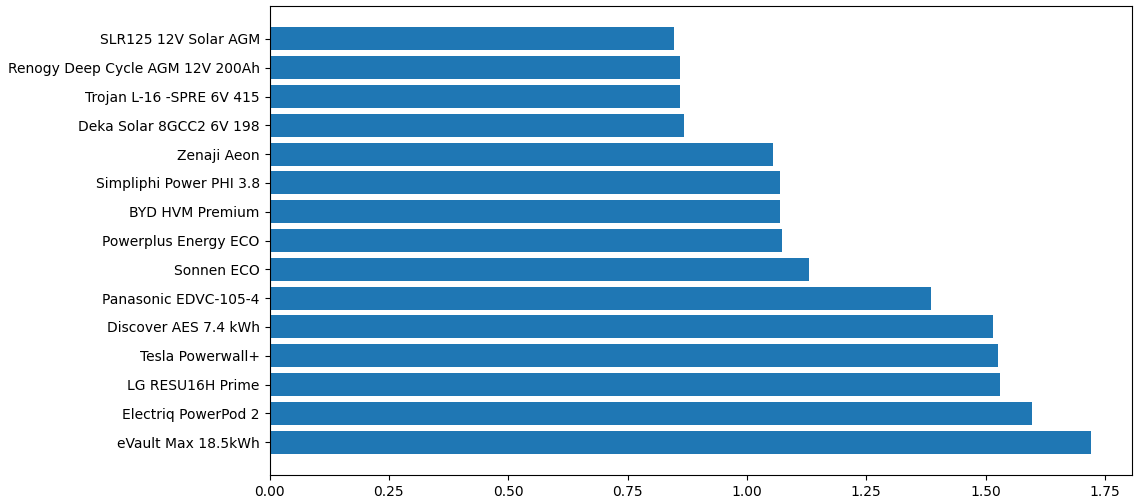
\includegraphics[scale=0.4]{src/3.png}
\end{figure}
In contrast, in several locations with extreme climates or households with many energy-intensive appliances, an increase in electrical usage is inevitable.
\begin{itemize}
    \item $L_a = 0.5 \text{days}$
\end{itemize}
In many situations, the location gets a lot of sunlight hours; therefore, the only occasion to discharge the battery is in the evening. In that case, the $L_a$ only last for 0.5 days:
\begin{figure}[H]
\centering
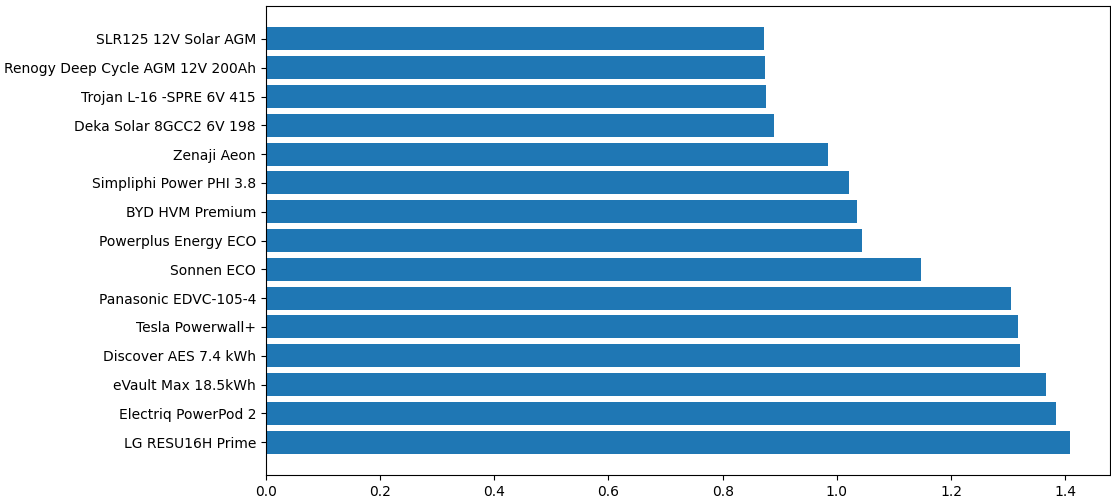
\includegraphics[scale=0.4]{src/4.png}
\end{figure}
\begin{itemize}
    \item $L_a \in \{2, 3\}$
\end{itemize}
There is a chance that there will be continuous periods of rain, so the solar system cannot capture enough energy, and you have to use the stored battery energy:
\begin{itemize}
    \item $L_a = 2:$
\end{itemize}
\begin{figure}[H]
\centering
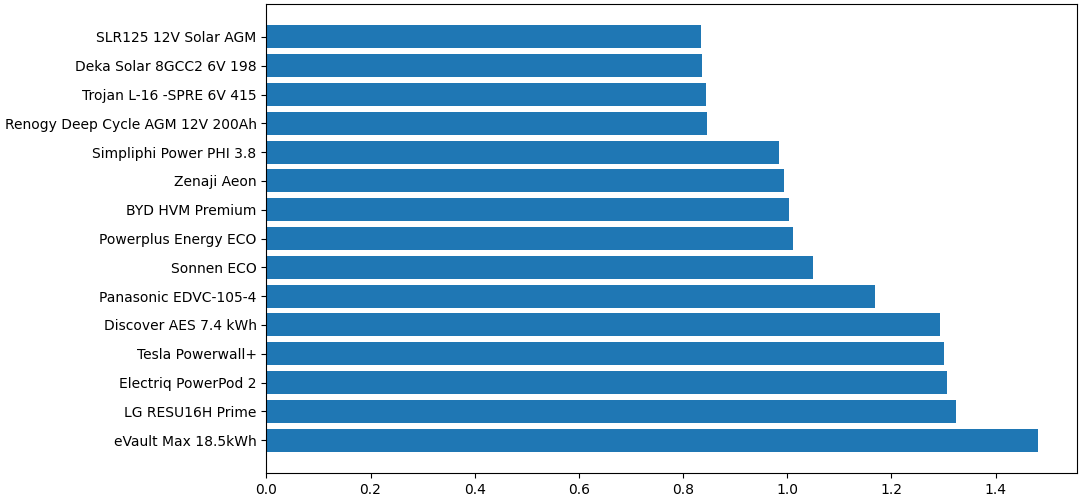
\includegraphics[scale=0.4]{src/5.png}
\end{figure}
\begin{itemize}
    \item $L_a = 3:$
\end{itemize}
\begin{figure}[H]
\centering
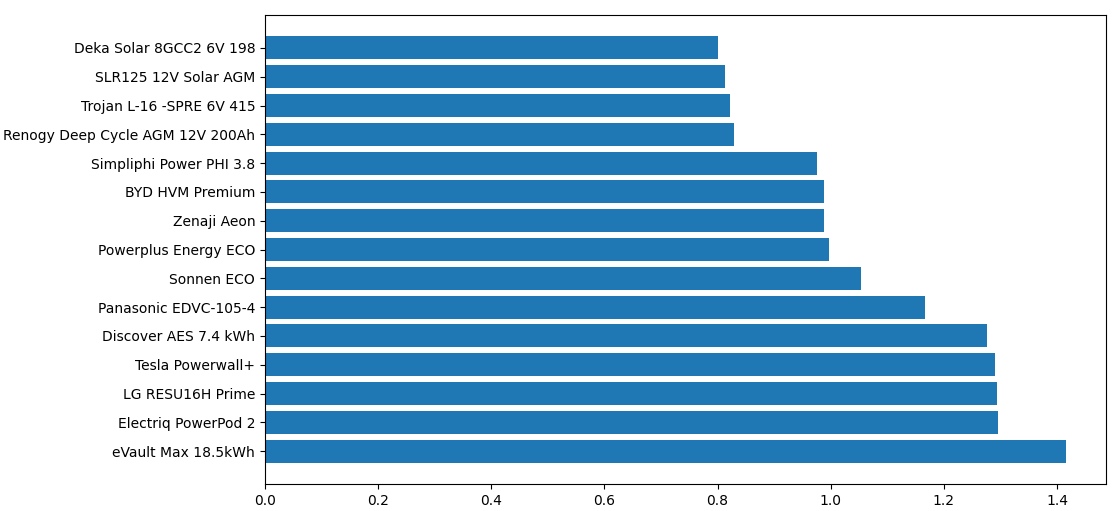
\includegraphics[scale=0.4]{src/6.png}
\end{figure}
Similar to the assumption above, we changed the state of health of all batteries to another similar value to compare more easily. However, some batteries have their lifetime inverse to their state of health's efficiency. Therefore, the assumption of the state of health will require several alterations.
\begin{itemize}
    \item $SoH = 80\%$
\end{itemize}
\begin{figure}[H]
\centering
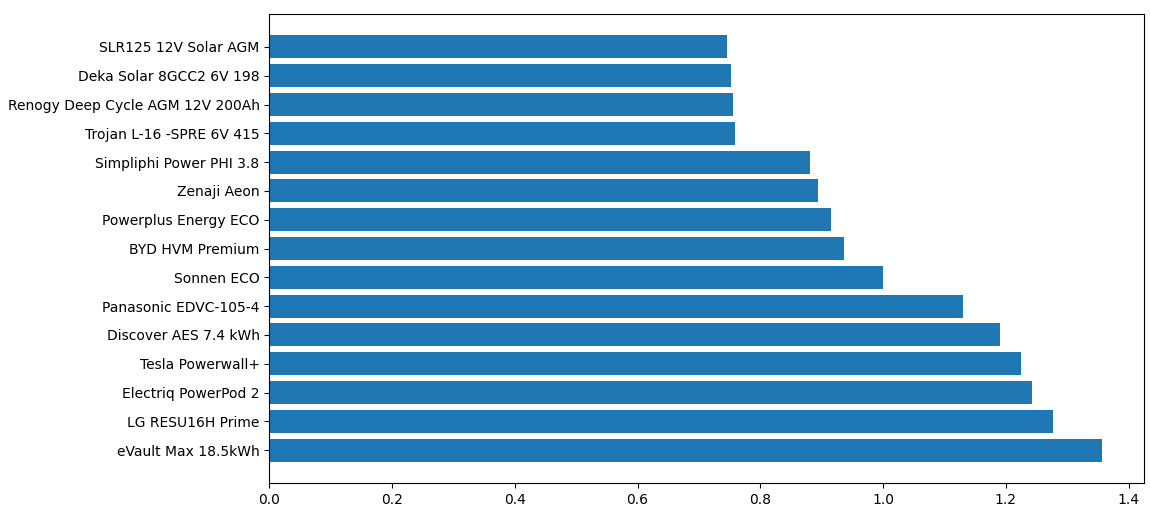
\includegraphics[scale=0.4]{src/7.png}
\end{figure}
\section{Evaluation}
The proportions contributing to the general rating can be changed easily, and we decided to make some adjustments to select the most accurate model. In addition, since the priorities of each person when installing a battery storage system are different, this ratio will adapt to different circumstances. In the end, we decided to alter several factors by increasing the cost rating to around 30\%-35\% and decreasing the capacity an equivalent amount, changing the lifetime rating and changing several formulas, et cetera. This results in what we believe to be the "best" model; however, the term "best" is relativistic, and other people may hold different views on what the "best" model is. We acknowledge that and respect their decisions, though our team has faith in the model's accuracy.

\section{Cement Batteries}
In 2021, researchers Emma Zhang and Luping Tang from Chalmers University of Technology, Gothenburg, Sweden\cite{buildings11030103} have discovered that cement can act as a medium to store and expend electricity (i.e. a rechargeable battery). By selecting iron (Fe) and zinc (Zn) as anodes, and nickel (Ni) oxides as cathodes, they determined that the best performance of the cement battery was the Ni-Fe battery, with short carbon fiber (CF) being added into the cement to modify the conductivity of the cement-based electrolytes,

In this part, we shall discuss the advantages and disadvantages that these batteries may possess, a possible way to implement the battery in our 1600 square-foot home and additional information required in order to solve more questions.
\subsection{Advantages}
When assessing the benefits that cement batteries may potentially bring to home users, we discover that cement batteries have multiple advantages over either lead-acid or lithium-ion batteries:
\begin{enumerate}
    \item Installation location
\end{enumerate}
In addition, some criteria need to be addressed concerning the storage cells where the batteries will be installed for traditional lead-acid batteries or lithium-ion batteries. For example, many lead-acid batteries require more space and need to be stored in a well-ventilated area; lithium-ion batteries need to be installed in a cool and heat-conductive location to mitigate the risk of overheating. On the other hand, cement-based batteries, which are installable inside walls, do not take up additional space. This may contribute to the next advantage:

\begin{enumerate}[resume]
    \item Cement batteries come pre-installed
\end{enumerate}
When installing a solar battery storage system, homeowners have to consider multiple factors, including energy demands, costs, lifetime, et cetera. Nevertheless, when installing cement batteries within the house, the architect and electrician have to plan the integration of such a system. As a result, when the homeowner decides to reside in the house, the system will be readily available, reducing the need for further adjustments.

\subsection{Disadvantages}
Concerning the drawbacks of such a system, many problems may arise during the installation, usage and maintenance process. Here are a few examples that our team has gathered:
\begin{enumerate}
    \item Scalability
\end{enumerate}
In the study above, Emma Zhang and Luping Tang used coated-metal electrodes with a dimension of 100 mm $\times$ 100 mm $\times$ 4 mm, while the size of the metal-coated CF meshes was 90 mm $\times$ 90 mm $\times$ 1 mm. However, when installing cement batteries in walls, the CF meshes' sizes will have to be scaled up, causing problems in scalability that manufacturers have to overcome.

\begin{enumerate}[resume]
    \item Difficulty to install in vertical walls
\end{enumerate}
The diagram below illustrates the method the researchers used to construct their model:
\begin{figure}[H]
\centering
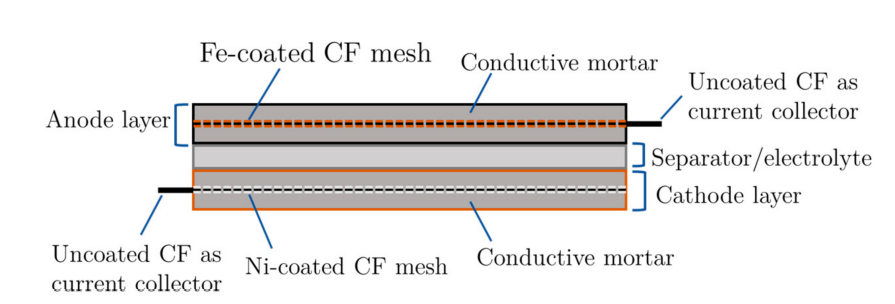
\includegraphics[scale=0.75]{A}
\caption{The 'sandwich' model utilised in cement batteries}
\label{fig:bat}
\end{figure}
The researchers had to embed the metal-coated CF mesh within the cement for the battery to function. When pouring cement into the cast, it had to be spread out into thin layers so that the results would be consistent. However, during the construction of a vertical wall, each concrete brick will be laid out alternatingly with steel beams before grout concrete is poured between the spaces to strengthen the wall.
\begin{figure}[H]
\centering
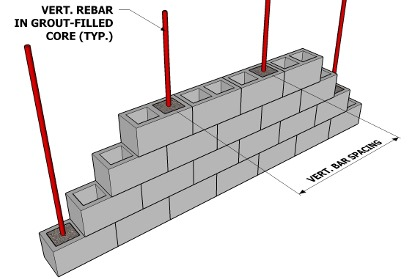
\includegraphics[scale=0.75]{B}
\caption{Construction of concrete walls}\cite{theconstructor:walls}
\end{figure}
This will lead to difficulties during both the construction of walls and the installation of cement batteries, which have not been solved yet.

\begin{enumerate}[resume]
    \item Maintenance issues
\end{enumerate}
If concrete walls are constructed using the above method, it will be impossible to investigate troubles that may arise during the maintenance process without harming the internal structures of the building. Consequently, parts of the wall will have to be destroyed and rebuilt to fix issues. In summary, the maintenance process will be costly and potentially be disruptive to both the electric grid and the family.
\subsection{Incorporation details}
After looking at the advantages and disadvantages of cement batteries, we have brainstormed and established details regarding incorporating cement batteries within a photovoltaic system. First, these batteries will only be installed on the floors and the ceilings. We require additional research and experiments before the feasibility of installing cement batteries in vertical walls can be determined. Therefore, in the following diagram, the battery can be implemented inside the concrete slab, between the insulation layer and damp-proof membrane:
\begin{figure}[H]
\centering
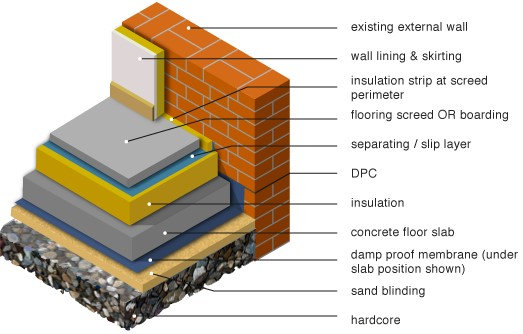
\includegraphics[scale=0.75]{C}
\caption{A breakdown of the structure of concrete floors}\cite{property:floor}
\end{figure}
By having two pieces of uncoated CF as current collectors as presented in Figure~\ref{fig:bat}, we can direct the current through an inverter, which will then supply energy to electric appliances within the house. In addition, the multiple floors and ceilings inside the home will allow more electricity to be stored, thus possibly powering the entire house on its own.
\subsection{Additional information}
We believe there are additional requirements that are important to a photovoltaic system but have not been addressed yet in the research above. By obtaining more data on these values, we can determine the feasibility of integrating cement batteries in solar-powered households:
\begin{enumerate}
    \item Battery lifetime
\end{enumerate}
As cement batteries are possibly difficult to maintain and replace, the lifetime of cement batteries is one of the most important factors, as fewer repairs are equivalent to less average cost over time. Therefore, more research on the lifespan of these batteries using different combinations of anode/cathode and multiple conditions is needed.
\begin{enumerate}[resume*]
    \item Cost of installation
\end{enumerate}
Since users want to minimise the cost of installation when installing solar batteries, if the correlation between house size, energy demand per day and cost of installation and maintenance can be determined, we will be able to assess the benefits of cement batteries with more clarity.

\begin{enumerate}[resume*]
    \item Power ratings 
\end{enumerate}
Our mathematical model presented above calculates the rating of each battery listed through the formula\eqref{eq:-2}. Therefore, to effectively evaluate the cement battery through our model, the continuous and instantaneous power rating of the battery - which takes up to 30\% in our mathematical model -  should be addressed.

As such, although our research has addressed the energy density of the material, additional experiments on the battery are necessary for us to evaluate its effectiveness.

\section{News article}
\newpage
\date{\today}
\currentvolume{1}
\currentissue{1}

\SetPaperName{Solar Times:}

\SetHeaderName{Solar Times}

\SetPaperLocation{Florida}
\SetPaperSlogan{``Powered by solar power.''}
\SetPaperPrice{Zero Dollars}
\maketitle
\thispagestyle{fancy}

\begin{multicols}{3}

\headline{Solar batteries: Factors to consider when installing}

As solar power becomes increasingly popular as an alternative energy source, more people are having trouble installing a solar system, especially those who go off-grid. There are many factors to consider; however, one of the most important parts of your home's electrical system is the energy storage system: batteries. These devices provide a way to store your hard-earned solar energy, in addition to powering all the necessary electric appliances in your house. Therefore, it is crucial to understand all the details involved when installing a battery storage system.

First, there are the energy demands within your household. Every piece of electrical equipment requires electricity in one way or another, so if you plan to go solar, you need to calculate your total energy usage per day in kilowatt-hours (kWh). By calculating the power consumed and the number of hours used by each electric appliance in your house, you can measure the total energy required to power your home.

After doing the calculations, you need to choose a battery type for your array. The two most popular choices for general home usage are lead-acid batteries and lithium-ion batteries. While lead-acid batteries have existed for a long time and are reliable, lithium-ion batteries not only offer you more storage per dollar you spend but also utilise solar energy with higher efficiency and depth of discharge (the percentage of power you consume from the battery) without quick degradation.

Next, you can start estimating the number of batteries required for your house. Either by using a solar battery calculator or calculating them by hand, you can adjust the number of batteries to purchase. You can also do this with other battery products to find the minimum cost of installation, which can save extra money.

In the end, after picking your desirable battery type, you can either hire an electrician to install your home circuit or rely on Internet guides to do that yourself. 
\closearticle

\headline{Cement batteries: A new future?}

Researchers from Gothenburg, Sweden have developed a battery model that incorporates the most common building material: cement. This allows previously unused wall space to be utilised as batteries, which may potentially revolutionise battery technology. By assessing the combinations of many common metals, the team has developed multiple batteries with metals embedded inside a concrete slab. After several testings, the researchers discovered that cement battery with nickel anode and iron cathode gives the best result: an average energy density of 7 Wh/m$^{2}$, or 0.8 Wh/L. Despite having a lower energy density than traditional solar batteries, researchers Emma Zhang and Luping Tang are optimistic about the possibility of "building rechargeable cement-based batteries on a large scale, with regards to the huge volume of a building." 

\closearticle

\end{multicols}
\restoregeometry

\pagestyle{fancy}
\newpage
\section{References}
%\LaTeX{} \cite{latex2e} is a set of macros built atop \TeX{} \cite{texbook}.
\bibliographystyle{unsrtnat}
\bibliography{src/cite/source} % Entries are in the refs.bib file


\section{Appendix}
\end{document}